\documentclass[10pt,a4paper]{article}
%\usepackage[pdftex, active, tightpage]{preview}
\usepackage[utf8]{inputenc}
\usepackage{amsmath}
\usepackage{amsfonts}
\usepackage{amssymb}
\usepackage[left=2cm,right=2cm,top=2cm,bottom=2cm]{geometry}

\usepackage{tikz}	%include TikZ-engine
\usepackage{mathpazo}
\usepackage{ifthen}
\usetikzlibrary{calc}

\begin{document}


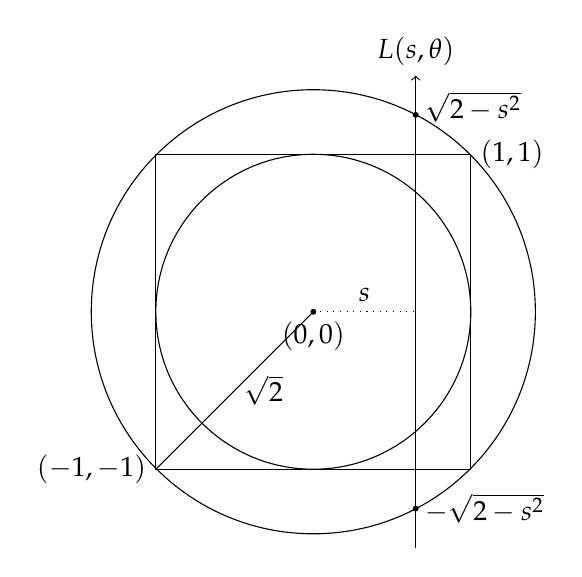
\begin{tikzpicture}
 

	\draw (-2,-2) rectangle (2,2);
	\draw (0.0,0) circle (2);
	\draw (0, 0) circle (2*1.41);	
	
	\draw[fill] (0,0) circle (0.03) node[right, below] {$(0,0)$};
	\draw[fill] (1.3, 2.5) circle (0.03);
	\draw[fill] (1.3, -2.5) circle (0.03);
	
	\draw (-2,-2) -- (0,0); 
	
	\draw[->] (1.3, -3) -- (1.3, 3) node[right, above] {$L(s,\theta)$};
	\draw[dotted] (0, 0) -- (1.3, 0);
	
	\node[right] at (1.3, -2.5) {$-\sqrt{2-s^2}$};
		\node[right] at (1.3, 2.6) {$\sqrt{2-s^2}$};
	
	\node[above] at (0.65, 0) {$s$};
	\node[right] at (-1, -1) {$\sqrt{2}$};
	\node[left] at (-2,-2) {$(-1, -1)$};
	\node[right] at (2,2) {$(1,1)$};
	
\end{tikzpicture}

\end{document}